\section{Camera Theory}

An image captured through a camera is the result of reflected light being detected on a cameras sensor, see figure \ref{fig:light_cam}. This process is know as \textit{image acquisition}. If you have no previous experience in image processing this might be mumbo-jumbo to you. In this chapter the basics of image acquisition using a digital camera will be explained. To understand this it is necessary to have a rudimentary understanding of the physics behind light.

\begin{figure}[htbp] 
\centering 
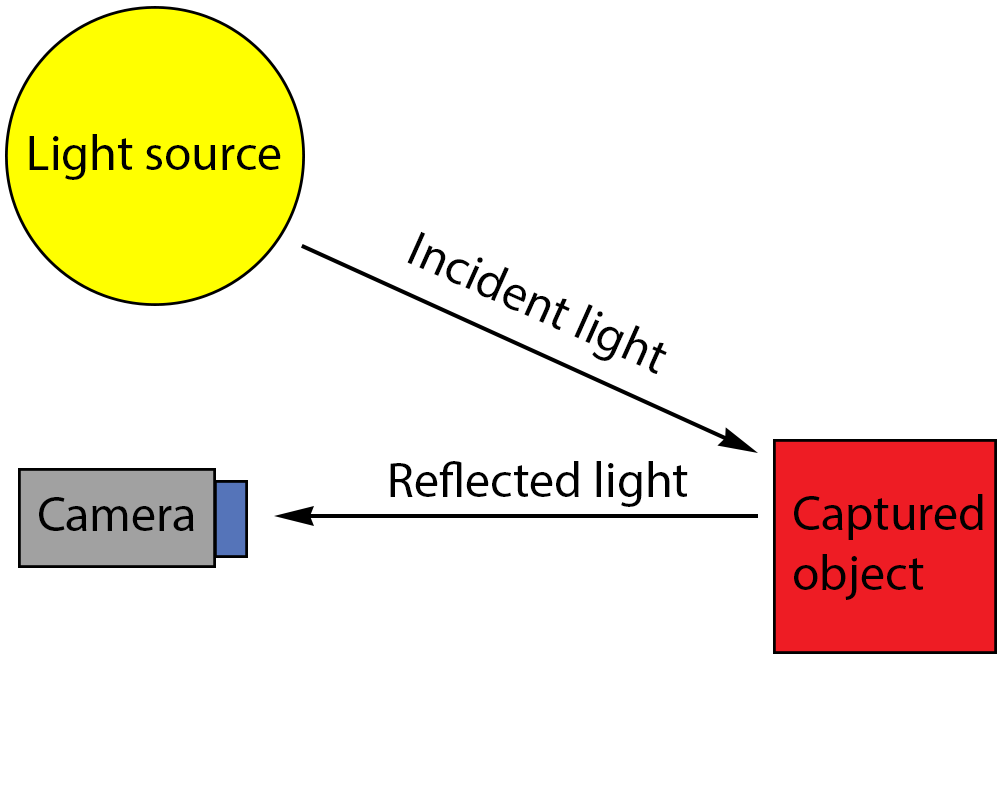
\includegraphics[width=0.5\textwidth]{Pictures/Theory/light_from_sun.png} 
\caption{Light as captured by a camera} 
\label{fig:light_cam} 
\end{figure}

Light is a form of electromagnetic radiation and can be viewed as both waves and particles. This duality is not something that we will be concerned with in this chapter. The wave model is sufficient to build the foundation of our understanding. A light wave is a small packet of energy travelling through space, these energy packet are known as photons. Photons can be described by three properties:

\begin{itemize}
\item \textbf{Wavelenght} - Measured in meters from wave top to wave top and denoted as $\lambda$.
\item \textbf{Frequency} - Measured in oscillations per second, Hz, denoted $f$.
\item \textbf{Energy} - Measured in electronvolts, eV, denoted $E$.
\end{itemize}

The formulae for these properties are as follows:

\begin{align}
\centering 
\lambda = \frac{C}{f}, \text{Where C is the speed of light}
\label{eq:wavelenght} 
\end{align}

\begin{align}
\centering
E = \frac{hC}{\lambda}, \text{Where h is Planck's constant}
\label{eq:e_v} 
\end{align}

The wavelenght of the photon determines what color you percieve, however as we know from physics, the speed of light is constant; thus changing the frequency will alter the color percieved. The visible spectrum of light is but a fraction of the full spectrum of electromagnetic radiation \fixme{SSEE THE FIGURE THAT IS NOT HTERE}. As with images, light interacts additively, with a mix of equal parts of each wavelenght resulting in white light.
\fixme{BILLEDE AF LYS i bølgelængder}
The most common light source by far is the sun. The white light we know from the sun can be broken down into it's component wavelenghts by refracting the light in a prism. This will yield the full color spectrum\fixme{MOAR PICTURES; LIGHT REFRACTED}
While different wavelengths correspond to different colors, these colors only remain defined within our perception. The reason we see 700nm light as red is because our eyes are constructed to be sensitive to three colors; red, green and blue. 
 


